\documentclass[11pt]{article}
\usepackage{fancyhdr}
\usepackage{graphicx}
\usepackage{float}
\usepackage{amssymb,amsmath}
\usepackage{psfrag}
\usepackage{color}
\usepackage[colorlinks]{hyperref}
\usepackage[footnotesize,hang,bf]{caption}
\usepackage{subeqnarray}
% \usepackage{amsthm}
 \usepackage{enumitem}
 \graphicspath{{Figures/}}
 \usepackage{multicol}
 \usepackage{ marvosym }
 \usepackage{wasysym}
 \usepackage{tikz}
 \usepackage[capitalize]{cleveref}
 \usetikzlibrary{patterns}

 \newcommand{\ds}{\displaystyle}
 \DeclareMathOperator{\sech}{sech}

%%%%%%%%%%%%%%%%%%%%%%%%%%%%%%%%%%%%%%%%%%%%%%%%%%%%%%%%%%%%%%%%%%%%%%%%%%%%%%%%%%

\def\term{Spring 2018}

\setlength{\oddsidemargin}{0 in}
\setlength{\evensidemargin}{0 in}
\setlength{\topmargin}{0.0 in}
\setlength{\textwidth}{6.45 in}
\setlength{\textheight}{8.5 in}
%\setlength{\headheight}{1 in}
\renewcommand{\baselinestretch}{0.95}

\pagestyle{fancy}
\rhead{ME 257/357\\ \term \\Mid-term Exam}
\lhead{}
\renewcommand{\headrulewidth}{0pt}

\begin{document}

\begin{center}
{\Large\bf ME 257/357 Gas Turbine Design: Mid-term\\
       Thursday, 5/24/2018, 10:30 - 11:50 am}
\end{center}

\hrule
\vspace{2mm}
%=======================================================================================================
\noindent Write your name on this handout and sign the honor code:

\vspace{6mm}
\noindent \textbf{Name}: \dotfill % \hfill\null
\vspace{2mm}

\noindent \textbf{Honor Code}: \emph{I have neither given nor received unauthorized aid on this examination, nor have I concealed any violations of the Honor Code.}

\vspace{6mm}
\noindent \textbf{Signiture}: \dotfill % \hfill\null 

\vspace{2mm}
\noindent This exam consists of two parts. Part 1 contains 10 short-answer problems (\emph{5 pts} each), and Part 2 contains 1 problem that requires detailed analysis to a turbofan engine. You need to complete both parts for full credit. Turn in both the blue book and this paper at the end of this exam.

\vspace{2mm}
\hrule

%=======================================================================================================
\vspace{2mm}

\section*{\textbf{PART 1} SHORT-ANSWERS (50 pts)} % (fold)
\label{sec:_textbf_part_1_short_answers}
\noindent \emph{This part is test your conceptual understanding of the course-material. Provide a brief but clear explanation or sketch for each question. Write or sketch the answer in the blue book.}

\begin{itemize}
	\item[(1)] Write down the equation of drag coefficient for a \emph{finite wing span}. Identify each term in the equation. Draw the drag polar.
	
	\item[(2)] Write down the thrust required in a steady level flight. Sketch $T^*$ as a function of the dynamic pressure $q_\infty$. Mark and define all asympototic lines on the plot.
	
	\item[(3)] What is the Breguet range equation? Sketch qualitatively the endurance factor and range factor as a function Mach number. Show curves at three different altitudes and explain why you draw it this way.
	
	\item[(4)] Draw the turbine solidification process on a phase diagram. Mark important points and curves on the diagram clearly.
	
	\item[(5)] What is a single crystal blade? Write down three advantages of using the single crystal technology for turbine blades.
	
	\item[(6)] Name three pollutent generated in the combustion process. Briefly explain how does each pollutent form and how to reduce it.
	
	\item[(7)] Draw a RQL combustor schematically. Identify the combustion processes on the sketch. Find the density of the gas simbolically in the dilution region. Clearly state all assumptions and definition of your simbols.
	
	\item[(8)] Define choke and stall in a compressor stage and explain their consequences.
	
	\item[(9)] Draw the compressor map qualitatively. Mark all important features on the graph.
	
	\item[(10)] Draw the turbine map qualitatively. Mark all important features on the graph.
	
\end{itemize}

% section _textbf_part_1_short_answers (end)

\newpage

\section{\textbf{PART 2} ENGINE ANALYSIS} % (fold)
\label{sec:_textbf_part_2_engine_analysis}
\noindent \emph{In this part of the exam you are asked to provide detailed analysis to the problem. Please write your derivations and mark the final results clearly.}

\subsection*{Low-order Design of a Turbofan Engine} % (fold)
\label{sub:low_order_design_of_a_turbofan_engine}
\noindent We will analyze a GE 90 turbofan engine (as shown in~\cref{fig:engine}) with efficiencies of each component listed in~\cref{tab:eff}. The free stream Mach number is $M_0 = 0.85$, temperature is $T_0 = 220$ K, and pressure is $P_0 = 24$ kPa. The core mass flow rate of air is $\dot{m}_a = 3.0$ kg/s, the bypass ratio is $2.9$, the fan pressure ratio is $2.0$.

\begin{figure}[ht]
	\centering
	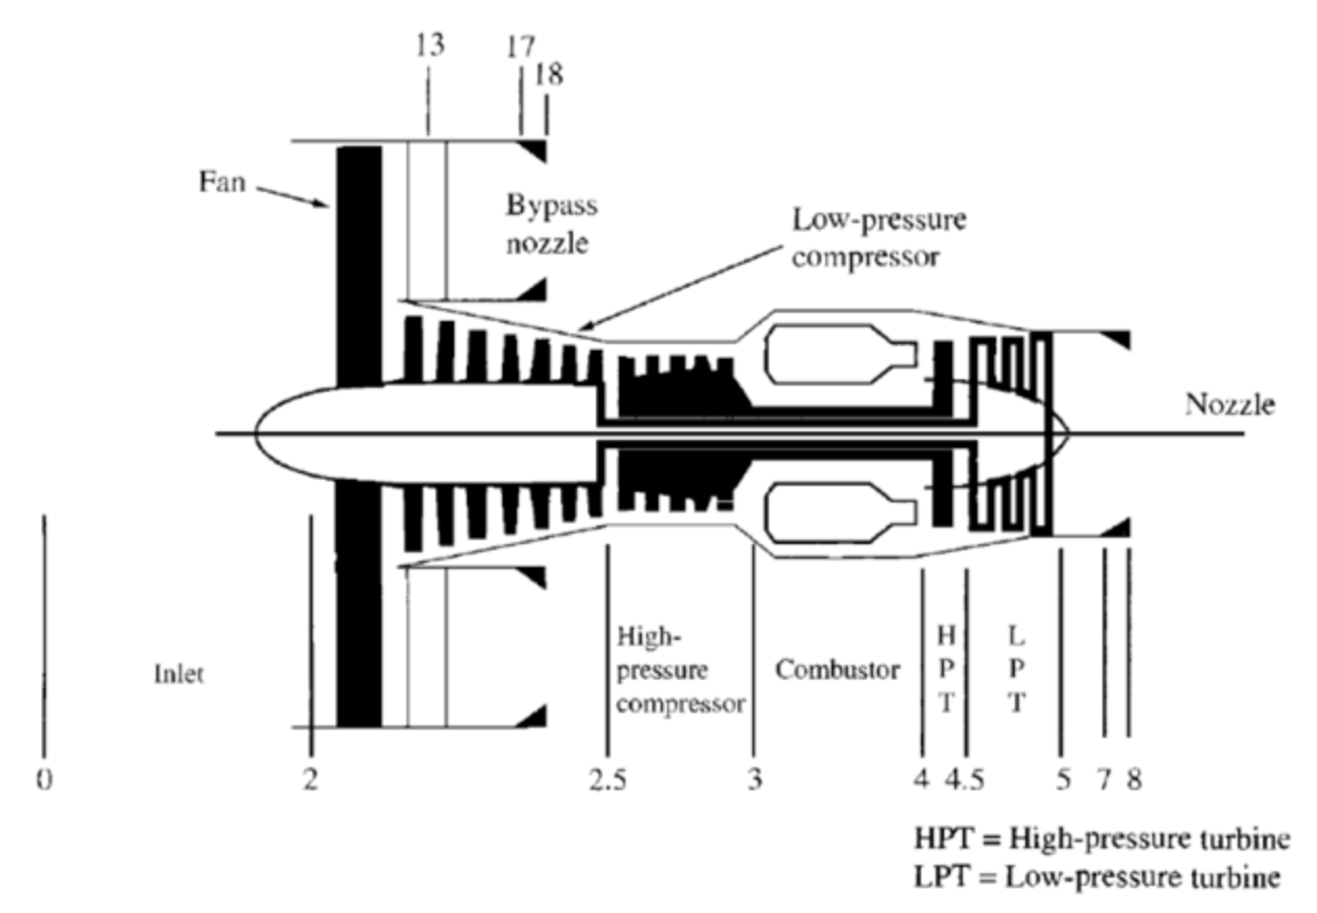
\includegraphics[width=\textwidth]{engine.pdf}
    \caption{Schematic of the GE90 engine with station numbering.}
	\label{fig:engine}
\end{figure}

\begin{table}[ht!]
	\caption{Turbofan component efficiencies.}
	\label{tab:eff}
	\centering
	\begin{tabular}{ | c | c |} 
			\hline
 		   	Component & $\eta_\text{adiabatic}$ \\ 
			\hline
			Diffuser & $95\%$ \\ 
			\hline
			Fan & $92\%$ \\
			\hline
			Compressor & $87\%$ \\
			\hline
			Combustor & $100\%$ \\
			\hline
			Turbine (LPT \& HPT) & $91\%$ \\
			\hline
			Core/Fan nozzle & $98\%$ \\
			\hline
	\end{tabular}
\end{table}

\begin{itemize}
	\item[(a)] \emph{Compressor analysis. (15 pts)} 
	\begin{itemize}
		\item (5 pts) For a single compressor stage (the first stage) shown in~\cref{fig:compressor}, complete the velocity triangle in~\cref{fig:compressor} across the rotor at the pitchline $r_m$. Assume the following quantities as known: the inlet velocity $U_{c1}$, the angle of attack of the flow after the inlet guide vain $\alpha_{c1}$, the angular velocity of the compressor $\Omega$, the relative angle at the rotor leading edge $\beta_{c1}$, and the relative angle at the rotor trailing edge $\beta_{c2}$. Express $U_{c1,\theta}$, $U_{c2,\theta}$, and $\alpha_{c2}$ using the known quantities.
		
		\begin{figure}[ht]
			\centering
			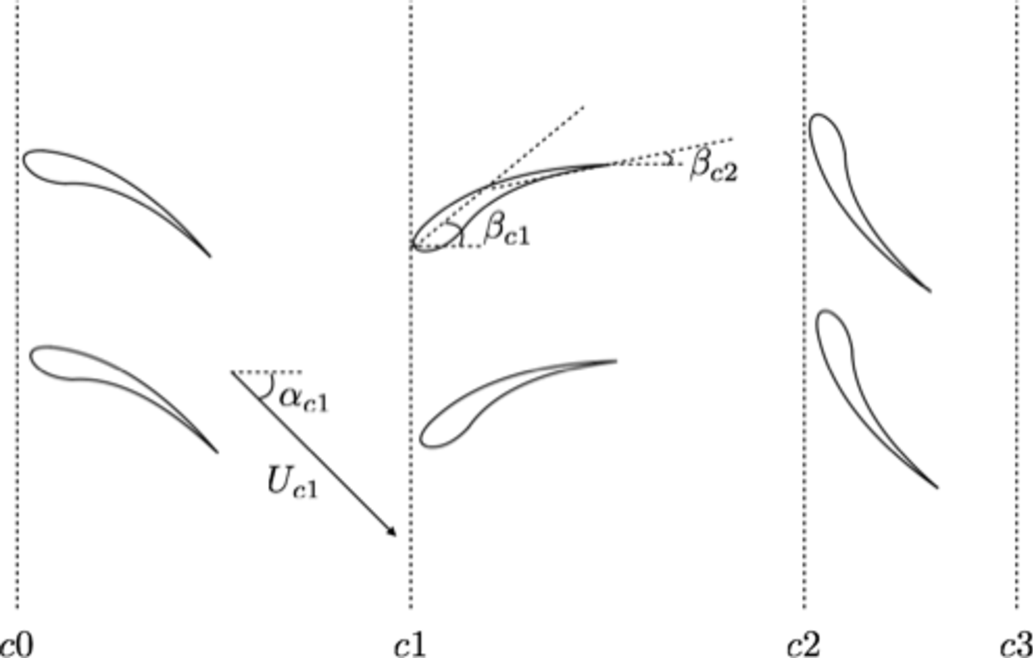
\includegraphics[width=\textwidth]{compressor.pdf}
		    \caption{Schematic of the the first compressor stage with station numbering.}
			\label{fig:compressor}
		\end{figure}
		
		\item (5 pts) What is the work comsumed by this compressor stage? Assuming the inlet velocity $U_{c1} = 150$ m/s, the vortex desgin follows the \emph{constant reaction} specification, the radius at the hub and the tip are $h_\text{hub} = 0.5$ m and $h_\text{tip} = 1.0$ m respectively.
		
		\item \emph{bonus (5 pts)}: what is the degree of reaction for this compressor stage?
		
		\item (5 pts) What is pressure ratio across this stage? Assuming there are 5 such stages, what is the pressure ratio provided by the compressor?
		
	\end{itemize}
	
	\item[(b)] \emph{Combustor analysis. (15 pts)}
	\begin{itemize}
		\item (5 pts) n-Hexadecane is used in the current engine. Write down the reaction equation for stoichiometry. What is the equivalence ratio in this combustor? Assuming the fuel-to-air ratio is $f=0.023$.
		
		\item (5 pts) What is the lower heating value of the reaction for the given fuel-to-air ratio?
		
		\item (5 pts) What is the stagnition temprature after the combustor, i.e. $T_{04}$?
		
	\end{itemize}
	
	\item[(c)] (14 pts) Perform the Brayton cycle analysis to the engine with station labeling shown in~\cref{fig:Ts}. Ignore the low-pressure compressor, i.e. the low-pressure turbine drives the fan only. Complete the T-s diagram with the numbers obtained from the cycle analysis. Mark each station clearly and draw addition constant pressure lines if necessary. Station 0 has been marked for you.
	
	\begin{figure}[ht]
		\centering
		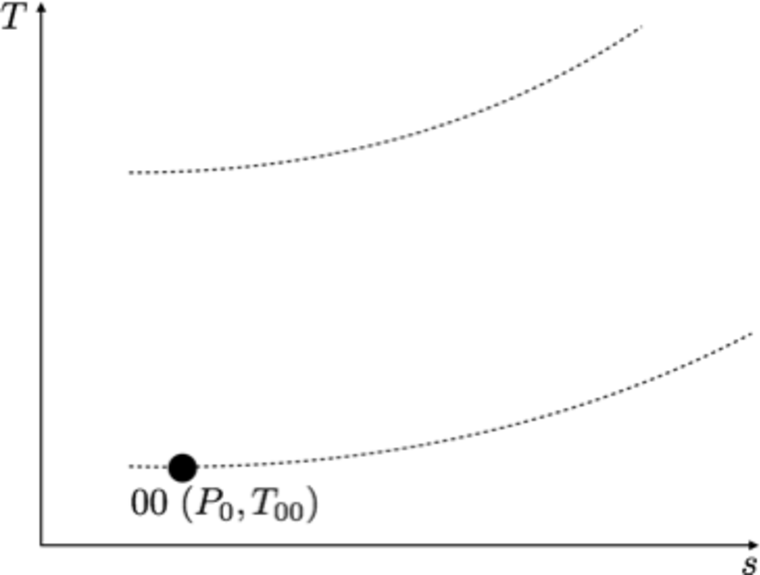
\includegraphics[width=\textwidth]{Ts_diagram.pdf}
	    \caption{T-s diagram of the Brayton cycle analysis to the GE90 engine.}
		\label{fig:Ts}
	\end{figure}
	
	\item[(d)] (6 pts) \emph{Engine Performance.}
	\begin{itemize}
		\item (3 pts) What is the thrust generated by the engine? What is the TSFC?
		
		\item (3 pts) What is the propulsive efficiency of the engine? At this part of the problem, assume $f\rightarrow 0$.
	\end{itemize}
		
\end{itemize}

% subsection low_order_design_of_a_turbofan_engine (end)

% section _textbf_part_2_detailed_analysis (end)

%=======================================================================================================
\end{document}
